% Chapter 6: Spectral Analysis
% ASSUMES: Chapter 5 defines H(s), H_z, H_0, |psi_0>, A_p, A_1, A_2,
%   s^*, delta_s, g_min, hat{g}, the three regions, symmetric states |k>,
%   eigenvalue equation (Lemma 5.1), validity of approximation (Lemma 5.2),
%   gap in window (Lemma 5.3), gap-left-preview (Lemma 5.4),
%   gap-right-preview (Lemma 5.5), Delta = E_1 - E_0.

Chapter 5 established the crossing window $\mathcal{I}_{s^*}$ where the spectral
gap satisfies $g(s) = \Theta(g_{\min})$, and it stated the outer-region bounds:
a linear lower bound on the left (\autoref{lem:gap-left-preview}) and on the
right (\autoref{lem:gap-right-preview}). What remains is to prove them.

The two proofs use different tools because the spectrum behaves differently on
the two sides of the crossing. To the left of $s^*$, the ground energy
$\lambda_0(s)$ sits below $sE_0$ while the first excited energy $\lambda_1(s)$
sits above it. A variational argument gives a sharp linear gap bound. To
the right of $s^*$, eigenvalues of $sH_z$ crowd the interval $[sE_0, sE_1]$,
and that variational strategy loses traction. There we switch to a resolvent
argument plus Sherman-Morrison for rank-one perturbations. The resulting profile
is steep on the left, flatter on the right, and nearly flat inside the window.

\section{Gap to the Left of the Crossing}
\label{sec:gap-left}

The eigenvalue equation (\autoref{lem:eigenvalue-equation}) places the ground
state energy at $\lambda_0(s) < sE_0$ and the first excited energy at
$\lambda_1(s) \in (sE_0, sE_1)$. This already proves $g(s) > 0$. It does not yet
give the quantitative lower bound needed for the runtime integral. What we need
is a bound that makes the left-side linear reopening explicit.

The strategy is to tighten the upper bound on $\lambda_0(s)$. Two routes give
the same linear form. The first uses the variational principle. For any
normalized state $\ket{\phi}$, the ground energy satisfies
$\lambda_0(s) \leq \bra{\phi}H(s)\ket{\phi}$, so a carefully chosen ansatz
directly yields a bound. The second uses concavity. Because
$\lambda_0(s) = \min_{\ket{\psi}} \bra{\psi} H(s) \ket{\psi}$ is the pointwise
minimum of affine functions in $s$, it is concave, and every tangent line lies
above it. We start with the variational route because it keeps the constants
explicit.

\begin{lemma}[Gap to the left of the crossing]
\label{lem:gap-left}
For any $s \in \mathcal{I}_{s^\leftarrow} = [0, \, s^* - \delta_s)$, the spectral gap of $H(s)$ satisfies
\begin{equation}
\label{eq:gap-left}
g(s) \geq \frac{A_1(A_1 + 1)}{A_2}\left(s^* - s\right).
\end{equation}
\end{lemma}

\begin{proof}
We upper-bound $\lambda_0(s)$ via the variational principle and lower-bound $\lambda_1(s)$ from the eigenvalue equation.

The ansatz must live in the span of $\{\ket{k} : k \geq 1\}$, orthogonal to the ground-state component $\ket{0}$, and should concentrate amplitude on levels close to $E_0$ where the energy expectation is lowest. The natural weighting is the inverse energy gap, because levels near $E_0$ should carry more amplitude. Unit normalization then fixes the scale, so we define
\begin{equation}
\label{eq:ansatz-left}
\ket{\phi} = \frac{1}{\sqrt{A_2 N}} \sum_{k=1}^{M-1} \frac{\sqrt{d_k}}{E_k - E_0}\,\ket{k}.
\end{equation}
This weighting also arises in first-order perturbation theory. The correction to the ground state $\ket{E_0}$ of $sH_z$ due to the perturbation $-(1-s)\ket{\psi_0}\bra{\psi_0}$ has coefficients proportional to $\braket{E_k}{\psi_0}/(E_k - E_0) = \sqrt{d_k/N}/(E_k - E_0)$, which matches the form above up to normalization. Normalization is immediate.
\begin{equation}
\braket{\phi}{\phi} = \frac{1}{A_2 N} \sum_{k=1}^{M-1} \frac{d_k}{(E_k - E_0)^2} = \frac{A_2}{A_2} = 1.
\end{equation}

To compute $\bra{\phi}H(s)\ket{\phi}$, decompose $H(s) = -(1-s)\ket{\psi_0}\bra{\psi_0} + s(H_z - E_0) + sE_0$. Each term contributes separately.

The projector term gives
\begin{equation}
-(1-s)\left|\braket{\psi_0}{\phi}\right|^2 = -(1-s)\left(\frac{1}{\sqrt{A_2 N}} \sum_{k=1}^{M-1} \frac{d_k}{(E_k - E_0)\sqrt{N}}\right)^{\!2} = -(1-s)\frac{A_1^2}{A_2},
\end{equation}
where $\braket{\psi_0}{\phi} = A_1/\sqrt{A_2}$ follows from $\braket{\psi_0}{k} = \sqrt{d_k/N}$ and the definition of $A_1$.

The shifted diagonal term gives
\begin{equation}
s\bra{\phi}(H_z - E_0)\ket{\phi} = \frac{s}{A_2 N} \sum_{k=1}^{M-1} \frac{d_k}{(E_k - E_0)^2} \cdot (E_k - E_0) = \frac{s}{A_2 N}\sum_{k=1}^{M-1} \frac{d_k}{E_k - E_0} = \frac{s\, A_1}{A_2}.
\end{equation}

The constant term contributes $sE_0 \braket{\phi}{\phi} = sE_0$. Combining the three terms gives
\begin{equation}
\label{eq:variational-bound}
\lambda_0(s) \leq \bra{\phi}H(s)\ket{\phi} = sE_0 - (1-s)\frac{A_1^2}{A_2} + s\frac{A_1}{A_2} = sE_0 + \frac{A_1}{A_2}\left(s(1 + A_1) - A_1\right).
\end{equation}
Since $s^*(1 + A_1) = A_1$, we have $s(1+A_1) - A_1 = (1+A_1)(s - s^*) = (s-s^*)/(1-s^*)$, so
\begin{equation}
\label{eq:lambda0-upper}
\lambda_0(s) \leq sE_0 + \frac{A_1}{A_2}\cdot\frac{s - s^*}{1 - s^*}.
\end{equation}
For $s < s^*$, the second term is negative, confirming $\lambda_0(s) < sE_0$.

For the first excited state, the eigenvalue equation (\autoref{lem:eigenvalue-equation}) confines $\lambda_1(s)$ to the interval $(sE_0, sE_1)$, so
\begin{equation}
\lambda_1(s) \geq sE_0.
\end{equation}

The gap is therefore
\begin{equation}
g(s) = \lambda_1(s) - \lambda_0(s) \geq sE_0 - sE_0 - \frac{A_1}{A_2}\cdot\frac{s - s^*}{1 - s^*} = \frac{A_1}{A_2}\cdot\frac{s^* - s}{1 - s^*}.
\end{equation}
Since $1/(1-s^*) = A_1 + 1$, we obtain $g(s) \geq A_1(A_1 + 1)(s^* - s)/A_2$.
\end{proof}

At the left boundary of the crossing window, $s = s^* - \delta_s$, the bound gives
\begin{equation}
g(s^* - \delta_s) \geq \frac{A_1(A_1+1)}{A_2}\cdot\delta_s = \hat{g},
\end{equation}
using $A_1(A_1+1)\delta_s/A_2 = \hat{g}$ from Eq.~\eqref{eq:gmin-deltas-relation}. Since $g_{\min} = (1 \pm O(\eta))\hat{g}$ from Eq.~\eqref{eq:gmin-formula}, the gap at the window boundary is $\Theta(g_{\min})$. The three-region decomposition is therefore tight because the left bound meets the window bound at the boundary rather than leaving a gap between them.

An alternative derivation uses concavity. Since $\lambda_0(s) = \min_{\ket{\psi}} \bra{\psi} H(s) \ket{\psi}$ is the pointwise minimum of affine functions in $s$, it is concave. The Hellmann-Feynman theorem \cite{Kato1950} gives the second derivative explicitly.
$$\ddot{\lambda}_0(s) = -2\sum_{j \geq 1} \frac{|\bra{\phi_j(s)}\dot{H}\ket{\phi_0(s)}|^2}{\lambda_j(s) - \lambda_0(s)} \leq 0,$$
where $\dot{H} = H_z + \ket{\psi_0}\bra{\psi_0}$ and $\ket{\phi_j(s)}$ are the instantaneous eigenstates. Concavity implies that every tangent line lies above the function. In particular, the tangent at $s^*$ gives $\lambda_0(s) \leq \lambda_0(s^*) + \lambda_0'(s^*)(s - s^*)$, an upper bound of the same form as~\eqref{eq:lambda0-upper}, though the variational approach gives slightly sharper constants.

When $M = 2$ ($d_0 = 1$, $d_1 = N-1$, $E_0 = 0$, $E_1 = 1$), the ansatz reduces to $\ket{\phi} = \ket{1}$, and the bound becomes
\begin{equation}
g(s) \geq \frac{(N-1)/N \cdot (2N-1)/N}{(N-1)/N}\left(\frac{1}{2} - s\right) = \frac{2N - 1}{N}\left(\frac{1}{2} - s\right) \approx 2\left(\frac{1}{2} - s\right).
\end{equation}
The exact gap $g(s) = \sqrt{(2s-1)^2 + 4s(1-s)/N}$ at $s = 1/4$ equals $\sqrt{1/4 + 3/(4N)} \approx 1/2$, while the bound gives $(2N-1)/(4N) \approx 1/2$. The bound is tight near $s^*$ and only becomes loose as $s$ approaches $0$, where the true gap approaches $1$ while the bound continues growing.

\section{Gap to the Right of the Crossing}
\label{sec:gap-right}

The variational principle cannot bound the gap to the right of $s^*$. It bounds ground energies from above, not excited energies from below, and what we need on the right is a lower bound on $\lambda_1(s) - \lambda_0(s)$ that captures the linear reopening of the gap.

The obstacle is structural. On the left, $\lambda_1(s)$ is bounded below by
$sE_0$ from the eigenvalue equation, which gives a clean anchor point. On the
right, $\lambda_1(s)$ still lies between $sE_0$ and $sE_1$, but now many higher
branches pass through the same interval and generate their own avoided
crossings. We need a method that controls spectral distance without tracking
individual branches one by one. The eigenvalue equation
(\autoref{lem:eigenvalue-equation}) characterizes the full spectrum implicitly,
but it does not directly give the linear-in-$(s-s^*)$ lower bound we need.

The resolvent provides exactly this. For a self-adjoint operator $A$ with spectrum $\sigma(A)$ and any $\lambda \notin \sigma(A)$, the resolvent
\begin{equation}
\label{eq:resolvent-def}
R_A(\lambda) = (\lambda I - A)^{-1}
\end{equation}
is a bounded operator whose norm equals the inverse distance from $\lambda$ to the spectrum:
\begin{equation}
\label{eq:resolvent-norm}
\lVert R_A(\lambda) \rVert = \frac{1}{\mathrm{dist}(\lambda,\, \sigma(A))}.
\end{equation}
This follows from the spectral theorem. In the eigenbasis of $A$ with
eigenvalues $\{\lambda_j\}$, the resolvent is diagonal with entries
$1/(\lambda - \lambda_j)$, so its operator norm is
$\max_j |1/(\lambda - \lambda_j)| = 1/\min_j|\lambda - \lambda_j|$. If a point
$\gamma$ lies between two consecutive eigenvalues $\lambda_0$ and $\lambda_1$,
then $\mathrm{dist}(\gamma, \sigma(A)) = \min(\gamma - \lambda_0, \lambda_1 -
\gamma) \leq g/2$, since the minimum of two non-negative numbers summing to $g$
is at most $g/2$. Therefore $\lVert R_A(\gamma) \rVert =
1/\mathrm{dist}(\gamma, \sigma(A)) \geq 2/g$, and the useful contrapositive is
\begin{equation}
\label{eq:gap-resolvent}
g(s) \geq \frac{2}{\lVert R_{H(s)}(\gamma) \rVert}.
\end{equation}
The spectral-gap problem has become a norm problem. A lower bound on the gap is
now an upper bound on a resolvent norm.

This resolvent approach to rank-one perturbations has precedent in spatial
search. Childs and Goldstone~\cite{childs2004spatial} used it to prove
$O(\sqrt{N})$ search time on the complete graph. Chakraborty, Novo, and
Roland~\cite{chakraborty2016spatial, chakraborty2020optimality} then extended
the method to broad graph families via Sherman-Morrison.

The algebraic structure is the same as in our Hamiltonian
$H(s) = sH_z - (1-s)\ket{\psi_0}\bra{\psi_0}$, with a graph Laplacian replaced
by a diagonal cost Hamiltonian. We therefore import the same mechanism, with
graph parameters replaced by $A_1$ and $A_2$.

Spatial search via continuous-time quantum walks asks for a marked vertex in a
graph $G$ on $N$ vertices by evolving
$\ket{s} = (1/\sqrt{N})\sum_v \ket{v}$ under
$H_{\text{search}} = -\gamma L - \sum_{v \in S}\ket{v}\bra{v}$, where $L$ is
the graph Laplacian and $\gamma > 0$ is tunable
\cite{childs2004spatial}. When $|S| = 1$, the oracle term is rank one (and low
rank more generally). The dictionary to our setting is direct. $L$ plays the
role of $sH_z$, the oracle projector plays the role of
$(1-s)\ket{\psi_0}\bra{\psi_0}$, the graph spectral gap corresponds to
$\Delta$, and effective resistance plays the role of $A_2$.

In both settings, one places a line $\gamma(s)$ between the two lowest
eigenvalues, applies Sherman-Morrison to split the resolvent into a known
diagonal part plus a correction term, and then bounds that correction. The
method works because rank-one perturbations of diagonal operators always admit
this inversion step, reducing the gap problem to one rational bound.

The constants $k = 1/4$ and $f(s^*) = 4$ are not accidents of this specific
Hamiltonian. They come from the same line-placement optimization that appears
whenever a rank-one perturbation is handled this way. The optimization balances
denominator positivity against numerator growth in $f(s)$. In that sense the
constants are structural. They do not depend on whether the unperturbed part is
a graph Laplacian or a diagonal cost Hamiltonian.

Since $H(s) = sH_z - (1-s)\ket{\psi_0}\bra{\psi_0}$ is a rank-one perturbation of $sH_z$, we can invert its resolvent explicitly. The Sherman-Morrison identity \cite{sherman_morrison} states that for an invertible operator $A$ and vectors $\ket{u}, \bra{v}$,
\begin{equation}
\label{eq:sherman-morrison}
(A + \ket{u}\bra{v})^{-1} = A^{-1} - \frac{A^{-1}\ket{u}\bra{v}A^{-1}}{1 + \bra{v}A^{-1}\ket{u}},
\end{equation}
provided $1 + \bra{v}A^{-1}\ket{u} \neq 0$. Applying this to the resolvent of $H(s)$ decomposes it into the resolvent of $sH_z$ (whose spectrum is known explicitly) and a correction from the rank-one term $-(1-s)\ket{\psi_0}\bra{\psi_0}$. The triangle inequality then yields an upper bound on $\lVert R_{H(s)}(\gamma)\rVert$.

We choose a line $\gamma(s)$ between $\lambda_0(s)$ and $\lambda_1(s)$ for all
$s \geq s^*$. Then we apply Sherman-Morrison, bound each contribution in terms
of $A_1$ and $A_2$, and convert the resulting resolvent estimate into a linear
lower bound on $g(s)$.

The simplest line starts at $sE_0$ when $s=s^*$ and ends between $E_0$ and
$E_1$ at $s=1$. Take $\beta(s)=a(s-s^*)/(1-s^*)$ with $a<\Delta$, and set
$\gamma(s)=sE_0+\beta(s)$. For $a=\Delta/6$, one can show $f(s)\le 1$ for all
$s\ge s^*$. This yields
$g(s)\ge \beta(s)= (\Delta/6)(s-s^*)/(1-s^*)$.
The bound is valid but too weak where the runtime is decided. At the window
boundary $s=s^*+\delta_s$, it gives
$g(s^*+\delta_s)\ge (\Delta/6)\cdot \delta_s/(1-s^*)
= (\Delta A_2)/(6A_1)\cdot g_{\min}$.
Since $\Delta A_2\le A_1$, this is at most $g_{\min}/6$, and it can be
polynomially smaller when $\Delta A_2\ll A_1$. At $s=s^*$, the same estimate
collapses to $g(s^*)\ge 0$, which misses the true minimum gap entirely.

The failure has a geometric explanation. At $s^*$, the ground energy
$\lambda_0(s^*)$ sits $g_{\min}/2$ below $s^*E_0$. The line $\gamma(s)$ passes
through $s^*E_0$ at $s=s^*$, so it has no safety margin from the lower branch.
At a midpoint between two eigenvalues, the resolvent norm is $2/g$. At a point
that touches one eigenvalue, it diverges. So the line must start at
$O(g_{\min})$ distance from both branches.

The fix is to shift the line origin from $s^*$ to a point $s_0 < s^*$ so that
$\beta(s^*) = k\, g_{\min}$ for a constant $k < 1$. With
$\beta(s) = a(s - s_0)/(1 - s_0)$, the constraint $\beta(s^*) = k\,g_{\min}$
determines
\begin{equation}
\label{eq:s0-definition}
s_0 = s^* - \frac{k\, g_{\min}(1 - s^*)}{a - k\, g_{\min}}.
\end{equation}
The line now passes through $\gamma(s^*) = s^*E_0 + k\,g_{\min}$, which lies between $\lambda_0(s^*)$ and $\lambda_1(s^*)$ when $k$ is chosen appropriately. The price is that $s_0 < s^*$ introduces extra terms in the monotonicity analysis for $f(s)$. We therefore need a careful choice of $a$.

\begin{lemma}[Gap to the right of the crossing]
\label{lem:gap-right}
Assume $A_1 \geq 1/2$. Let $k = 1/4$, $a = 4k^2\Delta/3 = \Delta/12$, and $s_0$ as in Eq.~\eqref{eq:s0-definition}. Then for all $s \geq s^*$, the spectral gap of $H(s)$ satisfies
\begin{equation}
\label{eq:gap-right}
g(s) \geq \frac{\Delta}{30}\cdot\frac{s - s_0}{1 - s_0}.
\end{equation}
\end{lemma}

\begin{proof}
Set $\gamma(s) = sE_0 + \beta(s)$ with $\beta(s) = a(s - s_0)/(1-s_0)$. The argument reduces to showing that a certain ratio $f(s)$, built from the numerator and denominator of the Sherman-Morrison correction, is monotonically decreasing on $[s^*,1]$. Once that is established, $\max_{s \geq s^*} f(s) = f(s^*) = O(1)$, and the resolvent bound $\lVert R_{H(s)}(\gamma)\rVert \leq (1/\beta)(1+f(s))$ converts directly into a linear gap lower bound.

Since $H(s) = sH_z - (1-s)\ket{\psi_0}\bra{\psi_0}$, the resolvent of $H(s)$ at $\gamma$ satisfies, via Eq.~\eqref{eq:sherman-morrison} and the triangle inequality,
\begin{equation}
\label{eq:resolvent-SM}
\lVert R_{H(s)}(\gamma)\rVert \leq \lVert R_{sH_z}(\gamma)\rVert + (1-s)\frac{\lVert R_{sH_z}(\gamma)\ket{\psi_0}\bra{\psi_0}R_{sH_z}(\gamma)\rVert}{1 + (1-s)\bra{\psi_0}R_{sH_z}(\gamma)\ket{\psi_0}}.
\end{equation}

The unperturbed resolvent $R_{sH_z}(\gamma)$ is diagonal in the $\ket{k}$ basis with entries $1/(\gamma - sE_k) = 1/(\beta - s(E_k - E_0))$ for $k \geq 1$ and $1/\beta$ for $k = 0$. The nearest eigenvalue of $sH_z$ to $\gamma$ is $sE_0$, at distance $\beta$, so $\lVert R_{sH_z}(\gamma)\rVert = 1/\beta$.

We now bound the numerator and denominator of the second term separately. Both
bounds use $\beta(s) \leq s(E_k - E_0)/2$ for all $k \geq 1$, so the Taylor
series in $\beta/(s(E_k - E_0))$ converges quickly. Here
$\beta(s) \leq a = \Delta/12$, while
$s(E_k - E_0) \geq s^*\Delta \geq \Delta/3$ because
$s^* = A_1/(A_1+1) \geq 1/3$ when $A_1 \geq 1/2$. Therefore
$\beta \leq \Delta/12 < \Delta/6 \leq s(E_k - E_0)/2$, as required.
The condition $A_1 \geq 1/2$ also marks the nontrivial search regime. Since
$A_1 \geq 1 - d_0/N$, the complementary case $A_1 < 1/2$ implies $d_0 > N/2$,
where random sampling already succeeds with constant probability.

\textbf{Numerator bound.} The squared norm of $R_{sH_z}(\gamma)\ket{\psi_0}$ expands as
\begin{equation}
\lVert R_{sH_z}(\gamma)\ket{\psi_0}\rVert^2 = \frac{d_0}{N\beta^2} + \frac{1}{N}\sum_{k=1}^{M-1}\frac{d_k}{\left(s(E_k - E_0) - \beta\right)^2}.
\end{equation}
Using $s(E_k - E_0) - \beta \geq s(E_k - E_0)/2$, each term in the sum is at most $4d_k/(Ns^2(E_k - E_0)^2)$, giving
\begin{equation}
\label{eq:numerator-bound}
\lVert R_{sH_z}(\gamma)\ket{\psi_0}\bra{\psi_0} R_{sH_z}(\gamma)\rVert \leq \lVert R_{sH_z}(\gamma)\ket{\psi_0}\rVert^2 \leq \frac{d_0}{N\beta^2} + \frac{4A_2}{s^2}.
\end{equation}

\textbf{Denominator bound.} Expanding the expectation value gives
\begin{align}
1 + (1-s)\bra{\psi_0}R_{sH_z}(\gamma)\ket{\psi_0} &= 1 + \frac{(1-s)d_0}{N\beta} - \frac{1-s}{N}\sum_{k=1}^{M-1}\frac{d_k}{s(E_k - E_0) - \beta} \nonumber \\
&= 1 + \frac{(1-s)d_0}{N\beta} - \frac{1-s}{s}\sum_{k=1}^{M-1}\frac{d_k}{N(E_k - E_0)}\sum_{\ell=0}^{\infty}\left(\frac{\beta}{s(E_k - E_0)}\right)^{\!\ell}.
\end{align}
Using $\beta/(s(E_k - E_0)) \leq 1/2$ to bound the geometric series by $1 + 2\beta/(s(E_k - E_0))$ gives
\begin{equation}
\label{eq:denominator-bound}
1 + (1-s)\bra{\psi_0}R_{sH_z}(\gamma)\ket{\psi_0} \geq 1 + \frac{(1-s)d_0}{N\beta} - (1-s)\left(\frac{A_1}{s} + \frac{2A_2\beta}{s^2}\right).
\end{equation}

\textbf{Collecting terms.} Substituting the bounds~\eqref{eq:numerator-bound} and~\eqref{eq:denominator-bound} into~\eqref{eq:resolvent-SM} and factoring gives
\begin{equation}
\label{eq:resolvent-f}
\lVert R_{H(s)}(\gamma)\rVert \leq \frac{1}{\beta}\left(1 + f(s)\right),
\end{equation}
and
\begin{equation}
\label{eq:f-definition}
f(s) = \frac{\frac{d_0}{N}\, s^2(1-s) + 4A_2\beta^2(1-s)}{\frac{d_0}{N}\, s^2(1-s) + \beta\, s\,\dfrac{s - s^*}{1 - s^*} - 2A_2\beta^2(1-s)}.
\end{equation}
To obtain this form, multiply numerator and denominator of the second term in~\eqref{eq:resolvent-SM} by $\beta$, then multiply by $s^2(1-s)$ to clear fractions. The key step is rewriting the denominator's constant-plus-linear terms using $A_1 = s^*/(1-s^*)$:
\begin{equation}
1 - \frac{(1-s)A_1}{s} + \frac{(1-s)d_0}{N\beta} = \frac{s - s^*}{s(1-s^*)} + \frac{(1-s)d_0}{N\beta},
\end{equation}
since $1 - A_1(1-s)/s = (s - A_1(1-s))/s = (s - s^*(1-s)/(1-s^*))/s = (s(1-s^*) - s^*(1-s))/(s(1-s^*)) = (s-s^*)/(s(1-s^*))$. Multiplying through by $\beta s^2(1-s)$ and collecting the Taylor-bounded terms into the $A_2\beta^2$ contributions gives Eq.~\eqref{eq:f-definition}. The fraction $d_0/N$ measures the density of ground states in the computational basis.

The numerator of $f(s)$ measures how strongly the rank-one perturbation can amplify the resolvent norm. The $d_0/N$ term comes from the $\ket{0}$ component of $\ket{\psi_0}$, and the $A_2$ term comes from the excited components. The denominator records the opposing effect. As $\gamma$ moves away from the crossing, the factor $\beta\,s(s-s^*)/(1-s^*)$ increases and pushes the resolvent back down. This is why $f(s^*)$ is only $O(1)$ near the crossing and why $f(s)\to 0$ as $s$ approaches $1$.

From~\eqref{eq:resolvent-f} and~\eqref{eq:gap-resolvent}, the spectral gap satisfies
\begin{equation}
\label{eq:gap-via-f}
g(s) \geq \frac{2\beta(s)}{1 + f(s)} \geq \frac{2\beta(s)}{1 + \max_{s \geq s^*} f(s)}.
\end{equation}
If $f$ is monotonically decreasing on $[s^*, 1]$, then $\max_{s \geq s^*} f(s) = f(s^*)$, and the bound becomes $g(s) \geq 2\beta(s)/(1 + f(s^*))$, which is linear in $s - s_0$.

\textbf{Monotonicity of $f$.} We show $f'(s) < 0$ for $s \in [s^*, 1]$. Write
$f = u/v$, so the sign of $f'$ is the sign of $u'v - uv'$. The derivative algebra
is long, so it helps to name the structure before expanding. After cancellation,
three terms remain, which we label $T_1$, $T_2$, $T_3$. Terms $T_1$ and $T_3$ are negative. Term $T_2$ is positive and proportional to $(d_0/N)\,s_0$, which appears because the line origin is shifted below $s^*$. The real work is to show that $T_1$ alone dominates $T_2$ on all of $[s^*,1]$. The argument factors $T_1 + T_2$ and compares a convex quadratic in $s$ (from $T_1$) against a cubic $s(1-s)^2$ (from $T_2$). Both expressions are bounded by their values at $s^*$, and the spectral condition (Definition~\ref{def:spectral-condition}) ensures the quadratic term wins.
Write $f = u/v$ with
\begin{align}
\label{eq:uv-def}
u &= \frac{d_0}{N}\,s^2(1-s) + 4A_2\beta^2(1-s), \\
v &= \frac{d_0}{N}\,s^2(1-s) + \beta\,s\,\frac{s - s^*}{1-s^*} - 2A_2\beta^2(1-s). \nonumber
\end{align}
Then $f' = (u'v - uv')/v^2$, so the sign of $f'$ is determined by $u'v - uv'$.

Computing $u'$ and $v'$ using $\beta' = a/(1-s_0)$:
\begin{align}
u' &= \frac{4aA_2\beta}{1-s_0}(2 + s_0 - 3s) + \frac{d_0}{N}\, s(2 - 3s), \label{eq:u-prime} \\
v' &= \frac{a(3s^2 - 2s(s^* + s_0) + s^*s_0)}{(1-s_0)(1-s^*)} - \frac{2aA_2\beta}{1-s_0}(2 + s_0 - 3s) + \frac{d_0}{N}\,s(2-3s). \nonumber
\end{align}

Expanding $u'v$ and $uv'$ and taking the difference produces exact cancellation
of two terms. The canceled terms are
$(d_0/N)^2 s^3(2-3s)(1-s)$ and
$8a A_2^2\beta^3(1-s)(2+s_0-3s)/(1-s_0)$. The remainder has three terms
\cite{braida2024unstructured}:
\begin{align}
\label{eq:upv-uvp}
u'v - uv' =\;& \underbrace{-\frac{4aA_2\beta^2}{(1-s_0)(1-s^*)}\Big(s^2(1 + s_0 - s^*) - 2s\,s_0 + s^*s_0\Big)}_{T_1} \\
&+ \underbrace{\frac{12aA_2\frac{d_0}{N}\,\beta}{1-s_0}\,s(1-s)^2\,s_0}_{T_2} \nonumber \\
&\underbrace{- \frac{\frac{d_0}{N}\,s^2 a}{(1-s_0)(1-s^*)}\Big({-}s^2(s^* + s_0 - 1) + 2s\,s_0 s^* - s^*s_0\Big)}_{T_3}. \nonumber
\end{align}
Terms $T_1$ and $T_3$ are negative, while $T_2$ is positive. The positive term $T_2$ is the only one that contains $(d_0/N)\,s_0$, so it is exactly the cost of shifting the line origin below $s^*$. We now show that $T_1$ alone controls $T_2$.

Factor out $-4aA_2\beta/(1-s_0)$ from $T_1 + T_2$:
\begin{equation}
\label{eq:domination-argument}
-\frac{4aA_2\beta}{1-s_0}\left(\frac{\beta}{1-s^*}\Big(s^2(1+s_0-s^*) - 2s\,s_0 + s^*s_0\Big) - \frac{3d_0}{N}\,s_0\,s(1-s)^2\right).
\end{equation}
The quadratic
$s^2(1+s_0-s^*) - 2s\,s_0 + s^*s_0$
is convex in $s$ because $1+s_0-s^* > 0$, and here $s_0 < s^*$.
Its minimizer lies at $s_m < s^*$, so throughout $[s^*,1]$ it stays above its
value at $s^*$. At $s=s^*$ that value is
$s^*(1-s^*)(s^*-s_0)>0$.
The cubic $s(1-s)^2$ reaches its maximum at $s=1/3\le s^*$, so on
$[s^*,1]$ it also stays below its value at $s^*$.
Therefore the bracket in~\eqref{eq:domination-argument} is bounded below by its
value at $s=s^*$:
\begin{equation}
\frac{a(s^*-s_0)^2}{1-s_0} - \frac{3d_0}{N}\, s_0(1-s^*)^2.
\end{equation}
Using $s_0 \leq s^*$ and $s^*-s_0 = k\,g_{\min}(1-s^*)/(a - k\,g_{\min})$, this is positive whenever
\begin{equation}
\label{eq:a-constraint}
a < \frac{4}{3}k^2\frac{A_1}{A_2}.
\end{equation}
Since $\Delta A_2 \leq A_1$ and
$A_2 \leq \sum_{k \geq 1} d_k/(N(E_k-E_0)^2) \leq A_1/\Delta$,
the choice $a = (4/3)k^2\Delta$ satisfies~\eqref{eq:a-constraint}.
With this choice, $u'v - uv' < 0$ on $[s^*,1]$, so $f$ is monotonically
decreasing.

\textbf{Evaluating $f(s^*)$.} At $s = s^*$, $\beta(s^*) = k\,g_{\min}$. The term $\beta\,s(s-s^*)/(1-s^*)$ vanishes, so
\begin{equation}
f(s^*) = \frac{\frac{d_0}{N}\,{s^*}^2(1-s^*) + 4A_2 k^2 g_{\min}^2(1-s^*)}{\frac{d_0}{N}\,{s^*}^2(1-s^*) - 2A_2 k^2 g_{\min}^2(1-s^*)}.
\end{equation}
Replacing $g_{\min}$ by its leading-order expression $\hat{g} = 2s^*\sqrt{d_0/(NA_2)}$ from Eq.~\eqref{eq:gmin-formula} (valid up to a $(1 \pm O(\eta))$ factor that does not affect the final constant), we have $A_2 k^2 \hat{g}^2 = 4k^2{s^*}^2 d_0/N$. Substituting gives
\begin{equation}
\label{eq:f-at-sstar}
f(s^*) = \frac{1 + 16k^2}{1 - 8k^2}.
\end{equation}
For $k = 1/4$, $f(s^*) = (1 + 1)/(1 - 1/2) = 4$, so $1 + f(s^*) = 5$.

\textbf{Final bound.} From~\eqref{eq:gap-via-f},
\begin{align}
g(s) &\geq \frac{2\beta(s)}{1 + f(s^*)} = \frac{2a}{1 + f(s^*)}\cdot\frac{s - s_0}{1 - s_0}.
\end{align}
The prefactor evaluates to
\begin{equation}
\frac{2a}{1+f(s^*)} = \frac{2 \cdot (4/3)k^2\Delta}{1 + (1+16k^2)/(1-8k^2)} = \frac{4}{3}k^2\cdot\frac{1-8k^2}{1+4k^2}\cdot\Delta.
\end{equation}
The function $P(k) = (4/3)k^2(1-8k^2)/(1+4k^2)$ is maximized at $k_{\mathrm{opt}} = \frac{1}{2}\sqrt{\sqrt{3/2} - 1} \approx 0.237$, where $P(k_{\mathrm{opt}}) = \frac{1}{3}(5 - 2\sqrt{6}) \approx 0.034$. For $k = 1/4$:
\begin{equation}
P(1/4) = \frac{4}{3}\cdot\frac{1}{16}\cdot\frac{1/2}{5/4} = \frac{1}{30}.
\end{equation}
Therefore $g(s) \geq (\Delta/30)(s - s_0)/(1 - s_0)$.
\end{proof}

Specializing to $M = 2$ and $\Delta = 1$, the bound gives $g(s) \geq (1/30)(s - s_0)/(1 - s_0)$, where $s_0 = 1/2 - O(1/\sqrt{N})$ is close to $s^* \approx 1/2$ for large $N$. Near $s = 3/4$, the exact gap from Eq.~\eqref{eq:grover-gap} is $g(3/4) = \sqrt{1/4 + 3/(4N)} \approx 1/2$, while the bound gives approximately $(1/30)(1/4)/(1/2) = 1/60$. The bound is conservative by a factor of approximately $30$ but correctly captures the linear growth. This constant is the price of a clean, uniform bound valid for all problem Hamiltonians satisfying the spectral condition.

\section{The Complete Gap Profile}
\label{sec:complete-profile}

Combining the results of this chapter with those of Chapter 5, the spectral gap $g(s)$ is bounded below across all of $[0, 1]$.

\begin{theorem}[Complete gap profile]
\label{thm:complete-profile}
Let $H_z$ satisfy the spectral condition (Definition~\ref{def:spectral-condition}) and assume $A_1 \geq 1/2$ (equivalently $s^* \geq 1/3$). The spectral gap of $H(s) = -(1-s)\ket{\psi_0}\bra{\psi_0} + sH_z$ satisfies, for all $s \in [0, 1]$:
\begin{equation}
\label{eq:piecewise-bound}
g(s) \geq
\begin{cases}
\dfrac{A_1(A_1+1)}{A_2}\left(s^* - s\right), & s \in \mathcal{I}_{s^\leftarrow} = \left[0,\, s^* - \delta_s\right), \\[10pt]
g_{\min}, & s \in \mathcal{I}_{s^*} = \left[s^* - \delta_s,\, s^* + \delta_s\right], \\[10pt]
\dfrac{\Delta}{30}\cdot\dfrac{s - s_0}{1 - s_0}, & s \in \mathcal{I}_{s^\rightarrow} = \left(s^* + \delta_s,\, 1\right],
\end{cases}
\end{equation}
where $s_0 = s^* - k\,g_{\min}(1-s^*)/(a - k\,g_{\min})$ with $k = 1/4$ and $a = \Delta/12$.
\end{theorem}

\begin{proof}
The three cases follow from \autoref{lem:gap-in-window} (window, proved in Chapter 5), \autoref{lem:gap-left} (left), and \autoref{lem:gap-right} (right). The right bound holds for all $s \geq s^*$ and therefore covers $\mathcal{I}_{s^\rightarrow}$. The window bound $g(s) \geq g_{\min}$ is tighter than the right bound at $s^*$ but weaker far from the crossing.
\end{proof}

The right branch uses $\frac{s-s_0}{1-s_0}$, while the published paper \cite{braida2024unstructured} writes $\frac{s-s^*}{1-s_0} + \frac{s^*-s_0}{1-s_0}$ as two separate terms. These are identical: $s - s_0 = (s - s^*) + (s^* - s_0)$. The single-fraction form absorbs the constant offset $s^* - s_0$ into the numerator, which simplifies the piecewise statement without changing the bound.

The bounds match across region boundaries. At the left boundary $s = s^* - \delta_s$,
\begin{equation}
\frac{A_1(A_1+1)}{A_2}\cdot\delta_s = \hat{g} = \Theta(g_{\min}),
\end{equation}
so the left bound at the window boundary is $\Theta(g_{\min})$, consistent with the window bound. At $s = s^*$, the right bound gives $g(s^*) \geq 2\beta(s^*)/(1 + f(s^*)) = 2k\,g_{\min}/5 = g_{\min}/10$, which is below $g_{\min}$ by a constant factor but still $O(g_{\min})$. The window bound provides the tighter estimate $g(s^*) = g_{\min}$.

The piecewise bounds are intentionally asymmetric. The left arm is steep, and
the right arm is shallower. The variational method tracks the left slope
closely. The resolvent method gives a weaker slope but remains valid through the
spectral congestion on the right. Geometrically, the profile is a broad V
centered at $s^*$ with a narrow rounded minimum of width about $2\delta_s$. The
left slope is $A_1(A_1+1)/A_2$, which is $O(\mathrm{poly}(n))$ for Ising
instances. The right slope is $\Delta/(30(1-s_0))$, set by the problem gap
$\Delta$. At the endpoints, $g(0)=1$ for $H_0$ and $g(1)=\Delta$ for $H_z$.

\begin{figure}[H]
\centering
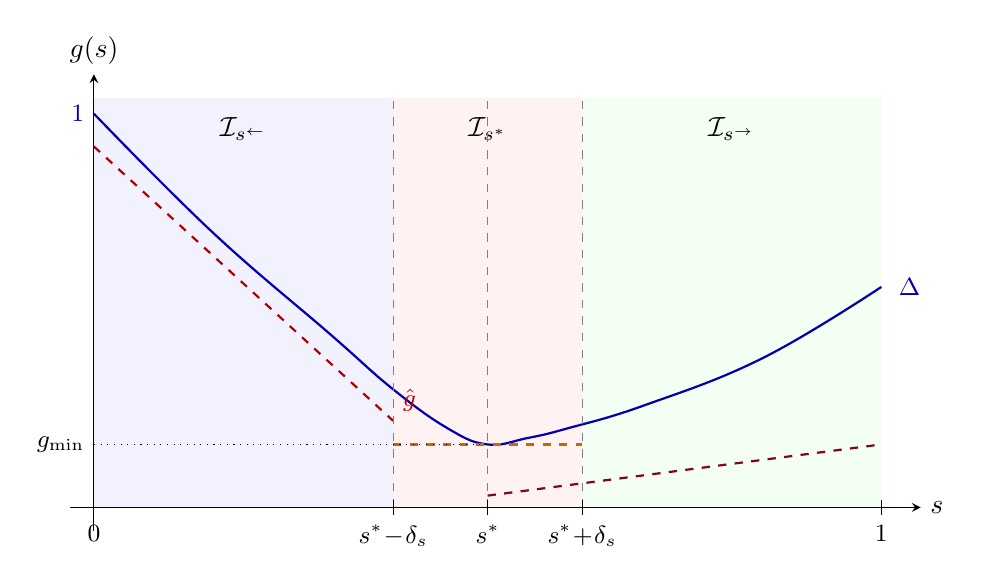
\begin{tikzpicture}[scale=1.0, >=stealth]
  % Axes
  \draw[->] (-0.3,0) -- (10.5,0) node[right] {$s$};
  \draw[->] (0,-0.3) -- (0,5.5) node[above] {$g(s)$};

  % Key positions
  \def\sstar{5.0}
  \def\dsl{1.2}
  \def\dsr{1.2}
  \def\gmin{0.8}
  \def\ghat{1.1}

  % Region shading
  \fill[blue!5] (0,0) rectangle (\sstar-\dsl,5.2);
  \fill[red!5] (\sstar-\dsl,0) rectangle (\sstar+\dsr,5.2);
  \fill[green!5] (\sstar+\dsr,0) rectangle (10,5.2);

  % Region labels
  \node at ({(\sstar-\dsl)/2}, 4.8) {$\mathcal{I}_{s^\leftarrow}$};
  \node at (\sstar, 4.8) {$\mathcal{I}_{s^*}$};
  \node at ({(\sstar+\dsr+10)/2}, 4.8) {$\mathcal{I}_{s^\rightarrow}$};

  % Exact gap (asymmetric: steep left arm, shallow right arm)
  \draw[thick, blue!70!black] plot[smooth, tension=0.7] coordinates {
    (0, 5.0)
    (1.5, 3.5)
    (3.0, 2.2)
    (3.8, 1.5)
    (4.5, 1.0)
    (\sstar, \gmin)
    (5.5, 0.88)
    (6.0, 1.0)
    (7.0, 1.3)
    (8.5, 1.9)
    (10, 2.8)
  };

  % Lower bounds (dashed)
  % Left: g(s) >= A_1(A_1+1)/A_2 * (s*-s), equals g_hat at s*-delta_s
  \draw[dashed, thick, red!70!black] (0, {(\sstar)*\ghat/\dsl}) -- (\sstar-\dsl, \ghat);

  % Window: horizontal at g_min
  \draw[dashed, thick, orange!80!black] (\sstar-\dsl, \gmin) -- (\sstar+\dsr, \gmin);

  % Right: g(s) >= Delta/30 * (s-s_0)/(1-s_0), slope controlled by Delta
  \draw[dashed, thick, purple!70!black] (\sstar, 0.15) -- (10, 0.80);

  % Vertical dashed lines at region boundaries
  \draw[thin, dashed, gray] (\sstar-\dsl, 0) -- (\sstar-\dsl, 5.2);
  \draw[thin, dashed, gray] (\sstar, 0) -- (\sstar, 5.2);
  \draw[thin, dashed, gray] (\sstar+\dsr, 0) -- (\sstar+\dsr, 5.2);

  % Tick marks
  \draw (0, 0.1) -- (0, -0.1) node[below, font=\small] {$0$};
  \draw (\sstar-\dsl, 0.1) -- (\sstar-\dsl, -0.1) node[below, font=\small] {$s^*\!-\!\delta_s$};
  \draw (\sstar, 0.1) -- (\sstar, -0.1) node[below, font=\small] {$s^*$};
  \draw (\sstar+\dsr, 0.1) -- (\sstar+\dsr, -0.1) node[below, font=\small] {$s^*\!+\!\delta_s$};
  \draw (10, 0.1) -- (10, -0.1) node[below, font=\small] {$1$};

  % g_min label
  \draw[thin, dotted] (0, \gmin) -- (\sstar, \gmin);
  \node[left, font=\small] at (0, \gmin) {$g_{\min}$};

  % g_hat label at window boundary
  \node[red!70!black, above right, font=\small] at (\sstar-\dsl, \ghat) {$\hat{g}$};

  % Endpoint values
  \node[blue!70!black, left, font=\small] at (0, 5.0) {$1$};
  \node[blue!70!black, right, font=\small] at (10.1, 2.8) {$\Delta$};
\end{tikzpicture}
\caption{Schematic gap profile for $H(s)$. The solid curve shows the true spectral gap $g(s)$, which equals $1$ at $s=0$, dips to $g_{\min}$ at $s = s^*$, and recovers to $\Delta$ at $s=1$. The left arm is steep (slope $A_1(A_1+1)/A_2$); the right arm is shallower (slope controlled by $\Delta$). Dashed lines show the piecewise lower bounds from \autoref{thm:complete-profile}: linear on the left, constant $g_{\min}$ in the window, and linear on the right (reaching $\Delta/30$ at $s=1$). The right bound is below $g_{\min}$ at $s^*$ but remains $O(g_{\min})$.}
\label{fig:gap-profile}
\end{figure}

Four parameters control the gap: $A_1$, $A_2$, $d_0$, and $\Delta$. For any problem Hamiltonian $H_z$ satisfying the spectral condition, \autoref{thm:complete-profile} bounds $g(s)$ over all of $[0,1]$ up to constants. The minimum is $g_{\min}=\Theta(\sqrt{d_0/(NA_2)})$ at $s^*=A_1/(A_1+1)$, and it is exponentially small in $n$ when $d_0=O(1)$. The crossing location depends only on $A_1$. More solutions (larger $d_0$) widen the gap, while richer near-ground spectral structure (larger $A_2$) narrows it. At $s=1$, the gap returns to $\Delta$, the spectral gap of $H_z$ itself.

For unstructured search, the exact gap $g(s) = \sqrt{(2s-1)^2 + 4s(1-s)/N}$ and the piecewise bound from \autoref{thm:complete-profile} can be compared directly. The left bound has slope $(2N-1)/N \approx 2$, matching the asymptotic slope of the exact gap, which approaches $2(1-1/N) \approx 2$ away from $s^*$. The window bound $g_{\min} = 1/\sqrt{N}$ is exact. The right bound has slope approximately $1/15$ near $s^*$, weaker than the true slope by a factor of $30$, but sufficient for the runtime integral since the window dominates.

The window dominates the runtime integral. $\int_0^1 g(s)^{-2}\,ds$ splits across the three regions. In the left and right regions, $g(s) \sim C|s - s^*|$ for constants $C$, and
\begin{equation}
\int_{\delta_s}^{s^*} \frac{du}{(Cu)^2} = \frac{1}{C^2}\left(\frac{1}{\delta_s} - \frac{1}{s^*}\right) \leq \frac{1}{C^2\delta_s},
\end{equation}
which is $O(1/(C^2\delta_s))$. In the window, $g(s) \geq g_{\min}$ gives $\int_{s^*-\delta_s}^{s^*+\delta_s} g(s)^{-2}\,ds \leq 2\delta_s/g_{\min}^2$. The window contribution $\delta_s/g_{\min}^2 = \Theta(A_2^{3/2}/(A_1(A_1+1)) \cdot \sqrt{N/d_0})$ dominates the outer regions. Once the $\Delta$-dependent right-arm term is included, the full integral yields the runtime
\[
T = O\!\left(\frac{\sqrt{A_2}}{A_1(A_1+1)\Delta^2}\sqrt{\frac{N}{d_0}}\right),
\]
which Chapter 7 derives rigorously.
